\subsection{Synthetic LP Benchmarks}

\begin{frame}{Synthetic LP Benchmarks}
    First, the paper considers two standard synthetic LP benchmarks.

    \begin{enumerate}
        \item \textbf{Shortest Path.} On a directed $5\times5$ grid, the model predicts 40 edge costs, and the downstream LP selects the minimum-cost path.
        \item \textbf{Knapsack.} The model predicts the values of 100 items. PEAR and LAVA use the LP relaxation during training, while all methods are evaluated on the original 0--1 problem.
    \end{enumerate}

    The feature vector is $\vx\sim\mathcal N(0,\mI_5)$, and the true costs are generated by a polynomial mapping with degree $\mathrm{deg}\in\{2,4,6,8\}$. Since the predictor is linear, a larger degree means a more nonlinear and harder prediction problem.

    \begin{itemize}
        \item Each task contains 1,000 training, 500 validation, and 500 test samples. Results are averaged over five random seeds.
        \item Baselines include two-stage MSE and four DFL methods: SPO+, PFYL, DBB, and LAVA.
        \item The metrics are normalized regret and training time. Additional tests inject multiplicative noise $\epsilon\in\{0.1,0.3,0.5\}$ into the cost mapping.
    \end{itemize}

    Thus, this experiment mainly tests whether PEAR can retain decision quality on LPs while computing the backward signal efficiently.

    \vfill
    {\tiny Source: \citet{lee2026decisionfocusedlearningtangentspaceprojection}, Sec.~5.1 and Apps.~C.1--C.2, E.1.}
\end{frame}

\begin{frame}{Synthetic LP Benchmarks}
    The following table keeps several representative settings from the full results.

    \begin{center}
        {\scriptsize
        \setlength{\tabcolsep}{3.8pt}
        \renewcommand{\arraystretch}{1.25}
        \begin{tabular}{llrrrr}
            \toprule
            Task & Deg. & \multicolumn{2}{c}{Regret (\%, $\downarrow$)} & \multicolumn{2}{c}{Time (s, $\downarrow$)}\\
            \cmidrule(lr){3-4}\cmidrule(lr){5-6}
                 & & PEAR & Best competitor & PEAR & Competitor\\
            \midrule
            Shortest Path & 4 & 0.774 & \textbf{0.761} (SPO+) & \textbf{23.5} & 41.8\\
            Shortest Path & 8 & \textbf{4.246} & 4.403 (SPO+) & \textbf{38.4} & 43.2\\
            Knapsack      & 4 & \textbf{0.315} & 0.381 (SPO+) & \textbf{305.2} & 600.0\\
            Knapsack      & 8 & \textbf{0.437} & 0.763 (SPO+) & \textbf{271.7} & 600.0\\
            \bottomrule
        \end{tabular}}
    \end{center}

    \small
    \begin{itemize}
        \item On Shortest Path, PEAR is best or tied at degrees 2, 6, and 8. At degree 4, SPO+ is slightly better in regret ($0.761$ versus $0.774$), but PEAR is about $1.8\times$ faster.
        \item On Knapsack, PEAR gives the lowest regret at every degree. At degree 8, its regret is $0.437$, compared with $0.763$ for SPO+; SPO+, PFYL, and DBB all reach the 600-second limit.
        \item Under multiplicative noise, PEAR remains best on both tasks. Even at $\epsilon=0.5$, it obtains regret $10.38$ on Shortest Path and $1.58$ on Knapsack.
    \end{itemize}

    In short, PEAR is best or tied in seven of the eight clean task--degree settings, with the clearest advantage on Knapsack and at larger polynomial degrees.

    \vfill
    {\tiny Source: \citet{lee2026decisionfocusedlearningtangentspaceprojection}, Tables~1--2.}
\end{frame}

\subsection{Real-World QP: Mean--Variance Optimization}

\begin{frame}{Real-World QP: Mean--Variance Optimization}
    Next, the paper considers a real-world QP based on S\&P 100 constituents from 2010--2024. The downstream problem is
    \begin{equation}
        \begin{aligned}
            \min_{\vw}\quad & \frac{\lambda}{2}\vw^\top\mSigma\vw-\hat{\vmu}^\top\vw\\
            \text{s.t.}\quad & \bm{1}^\top\vw=1,\qquad \vw\geq0,
        \end{aligned}
    \end{equation}
    where $\lambda=2.0$, so the optimizer constructs a fully invested, long-only mean--variance portfolio.

    \begin{itemize}
        \item DLinear with RevIN uses a 63-day return window to predict the next 21 days. The data are split chronologically into 70\% / 10\% / 20\%.
        \item The portfolio is rebalanced every 21 trading days, with a 0.1\% transaction cost applied to turnover.
        \item Baselines are two-stage MSE, QPTH, and CvxpyLayers. Evaluation includes regret, training time, returns, Sharpe ratio, and maximum drawdown.
    \end{itemize}

    For PEAR, OSQP is used in the forward pass to identify the active set, while the reduced-system backward pass is implemented through batched GPU linear algebra. This directly tests the computational claim from the previous section on a QP with $\mH=\lambda\mSigma$.

    \vfill
    {\tiny Source: \citet{lee2026decisionfocusedlearningtangentspaceprojection}, Sec.~5.2 and Apps.~C.3, E.2.}
\end{frame}

\begin{frame}{Real-World QP: Mean--Variance Optimization}
    Table~3 reports both optimization metrics and realized portfolio performance.

    \begin{center}
        {\scriptsize
        \setlength{\tabcolsep}{5.0pt}
        \renewcommand{\arraystretch}{1.28}
        \begin{tabular}{lrrrrrr}
            \toprule
            Method & Regret $\downarrow$ & Time $\downarrow$ & Cum. Ret. $\uparrow$ & Ann. Ret. $\uparrow$ & Sharpe $\uparrow$ & MDD $\uparrow$\\
                   & (\%) & (s) & (\%) & (\%) & & (\%)\\
            \midrule
            MSE          & 90.80 & \textbf{33.0} & 89.22  & 37.51 & 0.92 & -40.00\\
            QPTH         & 87.85 & 147.6 & 139.77 & 47.88 & 1.15 & -34.94\\
            CvxpyLayers  & 87.36 & 321.9 & 134.88 & 47.39 & 1.15 & -36.47\\
            \textbf{PEAR} & \textbf{85.38} & \textbf{122.3} & \textbf{184.19} & \textbf{58.84} & \textbf{1.44} & \textbf{-29.35}\\
            \bottomrule
        \end{tabular}}
    \end{center}
    {\footnotesize Means over five seeds; standard deviations are omitted for readability. For MDD, closer to zero is better.}

    \small
    \begin{itemize}
        \item PEAR gives the lowest regret, $85.38\%$, and is faster than both differentiable QP layers: 122.3 seconds versus 147.6 for QPTH and 321.9 for CvxpyLayers.
        \item It also gives the best realized portfolio metrics: cumulative return $184.19\%$, annualized return $58.84\%$, Sharpe ratio $1.44$, and maximum drawdown $-29.35\%$.
        \item MSE is the fastest because it does not differentiate through the downstream problem, but its decision quality and portfolio performance are worse.
    \end{itemize}

    Thus, in this experiment, lower decision-focused regret is accompanied by both higher realized return and better downside-risk control.

    \vfill
    {\tiny Source: \citet{lee2026decisionfocusedlearningtangentspaceprojection}, Table~3.}
\end{frame}

\subsection{Robustness Under Constraint Shifts}

\begin{frame}{Robustness Under Constraint Shifts}
    Finally, the paper asks whether the learned predictor still works when the downstream constraints change after training. The cost or return process is fixed, and only the feasible region is modified.

    \begin{center}
        {\small
        \setlength{\tabcolsep}{5pt}
        \renewcommand{\arraystretch}{1.30}
        \begin{tabular}{lll}
            \toprule
            Task & Training constraint & Test-time constraint\\
            \midrule
            Shortest Path & Directed corner-to-corner route & New origin--destination pair and edge direction\\
            Knapsack & Capacity ratio $\rho=0.5$ & $\rho\in\{0.3,0.5,0.7,0.9\}$\\
            Portfolio QP & Long-only ($\ell=0$) & $\ell\in\{-0.1,-0.3,-0.5,-1.0\}$\\
            \bottomrule
        \end{tabular}}
    \end{center}

    \begin{itemize}
        \item Shortest Path changes the routing direction and origin--destination pair on the same grid, testing whether the model learns edge costs rather than memorizing training paths.
        \item Knapsack changes the capacity ratio, making the feasible region tighter or looser. The main-text figure uses the tighter shift $0.5\to0.3$.
        \item Portfolio QP permits short selling through negative lower bounds. Unlike the first two representative shifts, this expands the feasible region.
    \end{itemize}

    For the LP tasks, the main comparison uses degree 8, i.e., the hardest polynomial setting. The metric is normalized regret under the shifted constraint.

    \vfill
    {\tiny Source: \citet{lee2026decisionfocusedlearningtangentspaceprojection}, Sec.~5.3 and Apps.~D, F.}
\end{frame}

\begin{frame}{Robustness Under Constraint Shifts}
    \begin{center}
        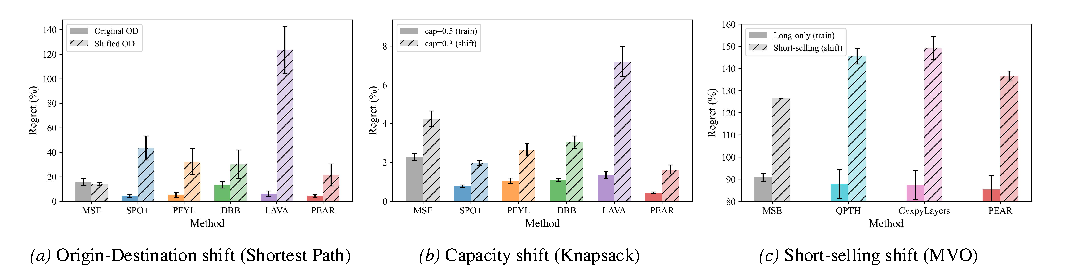
\includegraphics[width=0.88\linewidth]{figures/constraint_shifts.pdf}
    \end{center}
    \vspace{-0.4em}
    \footnotesize
    \begin{itemize}
        \item \textbf{Shortest Path.} MSE is best overall. Among DFL methods, PEAR degrades least, while SPO+, PFYL, DBB, and especially LAVA deteriorate substantially. This suggests that some DFL methods learn paths specialized to the training direction.
        \item \textbf{Knapsack.} PEAR gives the lowest regret when capacity tightens. The appendix shows the same pattern across the wider capacity sweep and all polynomial degrees.
        \item \textbf{Portfolio QP.} MSE is again best, while PEAR is the best DFL method. The DFL gap is smaller here, likely because the QP methods use closely related KKT information.
    \end{itemize}

    In short, PEAR is consistently the most robust method within the DFL family. However, MSE remains better on the Shortest Path and Portfolio shifts, so in-distribution decision quality and generalization to a new feasible region should be viewed separately.

    \vfill
    {\tiny Source: \citet{lee2026decisionfocusedlearningtangentspaceprojection}, Fig.~2 and Apps.~F.1--F.3.}
\end{frame}
